\begin{figure}[t]
\centering
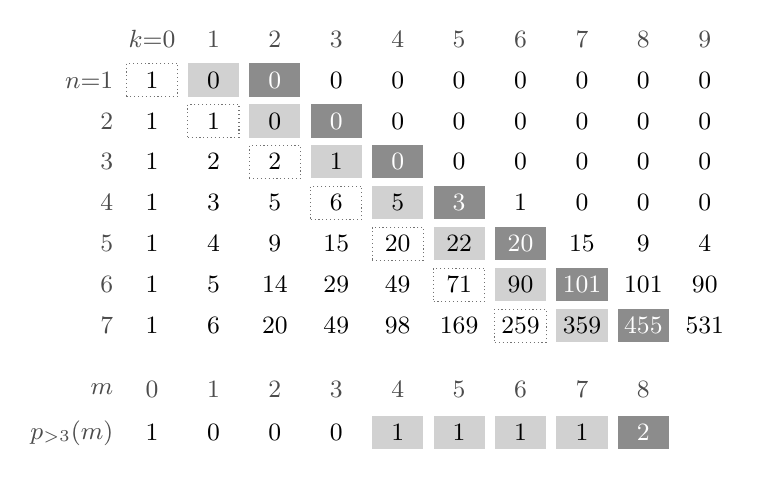
\begin{tikzpicture}[font=\small,
  plain/.style={minimum width=6.5mm,minimum height=4.2mm,inner sep=0pt},
  diag/.style={plain,fill=black!18},
  sub/.style={plain,draw=black!55,densely dotted},
  sup/.style={plain,fill=black!45,text=white},
  one/.style={plain,fill=black!18},
  two/.style={plain,fill=black!45,text=white},
  hdr/.style={inner sep=1pt,text=black!70}]
\node[hdr] at (0.00,0) {$k{=}0$}; \node[hdr] at (0.78,0) {1}; \node[hdr] at (1.56,0) {2}; \node[hdr] at (2.34,0) {3}; \node[hdr] at (3.12,0) {4}; \node[hdr] at (3.90,0) {5}; \node[hdr] at (4.68,0) {6}; \node[hdr] at (5.46,0) {7}; \node[hdr] at (6.24,0) {8}; \node[hdr] at (7.02,0) {9};
\node[hdr,anchor=east] at (-0.45,-0.52) {$n{=}1$}; \node[hdr,anchor=east] at (-0.45,-1.04) {2}; \node[hdr,anchor=east] at (-0.45,-1.56) {3}; \node[hdr,anchor=east] at (-0.45,-2.08) {4}; \node[hdr,anchor=east] at (-0.45,-2.60) {5}; \node[hdr,anchor=east] at (-0.45,-3.12) {6}; \node[hdr,anchor=east] at (-0.45,-3.64) {7};
\node[sub] at (0.00,-0.52) {1};
\node[diag] at (0.78,-0.52) {0};
\node[sup] at (1.56,-0.52) {0};
\node[plain] at (2.34,-0.52) {0};
\node[plain] at (3.12,-0.52) {0};
\node[plain] at (3.90,-0.52) {0};
\node[plain] at (4.68,-0.52) {0};
\node[plain] at (5.46,-0.52) {0};
\node[plain] at (6.24,-0.52) {0};
\node[plain] at (7.02,-0.52) {0};
\node[plain] at (0.00,-1.04) {1};
\node[sub] at (0.78,-1.04) {1};
\node[diag] at (1.56,-1.04) {0};
\node[sup] at (2.34,-1.04) {0};
\node[plain] at (3.12,-1.04) {0};
\node[plain] at (3.90,-1.04) {0};
\node[plain] at (4.68,-1.04) {0};
\node[plain] at (5.46,-1.04) {0};
\node[plain] at (6.24,-1.04) {0};
\node[plain] at (7.02,-1.04) {0};
\node[plain] at (0.00,-1.56) {1};
\node[plain] at (0.78,-1.56) {2};
\node[sub] at (1.56,-1.56) {2};
\node[diag] at (2.34,-1.56) {1};
\node[sup] at (3.12,-1.56) {0};
\node[plain] at (3.90,-1.56) {0};
\node[plain] at (4.68,-1.56) {0};
\node[plain] at (5.46,-1.56) {0};
\node[plain] at (6.24,-1.56) {0};
\node[plain] at (7.02,-1.56) {0};
\node[plain] at (0.00,-2.08) {1};
\node[plain] at (0.78,-2.08) {3};
\node[plain] at (1.56,-2.08) {5};
\node[sub] at (2.34,-2.08) {6};
\node[diag] at (3.12,-2.08) {5};
\node[sup] at (3.90,-2.08) {3};
\node[plain] at (4.68,-2.08) {1};
\node[plain] at (5.46,-2.08) {0};
\node[plain] at (6.24,-2.08) {0};
\node[plain] at (7.02,-2.08) {0};
\node[plain] at (0.00,-2.60) {1};
\node[plain] at (0.78,-2.60) {4};
\node[plain] at (1.56,-2.60) {9};
\node[plain] at (2.34,-2.60) {15};
\node[sub] at (3.12,-2.60) {20};
\node[diag] at (3.90,-2.60) {22};
\node[sup] at (4.68,-2.60) {20};
\node[plain] at (5.46,-2.60) {15};
\node[plain] at (6.24,-2.60) {9};
\node[plain] at (7.02,-2.60) {4};
\node[plain] at (0.00,-3.12) {1};
\node[plain] at (0.78,-3.12) {5};
\node[plain] at (1.56,-3.12) {14};
\node[plain] at (2.34,-3.12) {29};
\node[plain] at (3.12,-3.12) {49};
\node[sub] at (3.90,-3.12) {71};
\node[diag] at (4.68,-3.12) {90};
\node[sup] at (5.46,-3.12) {101};
\node[plain] at (6.24,-3.12) {101};
\node[plain] at (7.02,-3.12) {90};
\node[plain] at (0.00,-3.64) {1};
\node[plain] at (0.78,-3.64) {6};
\node[plain] at (1.56,-3.64) {20};
\node[plain] at (2.34,-3.64) {49};
\node[plain] at (3.12,-3.64) {98};
\node[plain] at (3.90,-3.64) {169};
\node[sub] at (4.68,-3.64) {259};
\node[diag] at (5.46,-3.64) {359};
\node[sup] at (6.24,-3.64) {455};
\node[plain] at (7.02,-3.64) {531};
\node[hdr,anchor=east] at (-0.45,-4.45) {$m$};
\node[hdr,anchor=east] at (-0.45,-5.0) {$p_{>3}(m)$};
\node[plain] at (0.00,-5.0) {1}; \node[hdr] at (0.00,-4.45) {0}; \node[plain] at (0.78,-5.0) {0}; \node[hdr] at (0.78,-4.45) {1}; \node[plain] at (1.56,-5.0) {0}; \node[hdr] at (1.56,-4.45) {2}; \node[plain] at (2.34,-5.0) {0}; \node[hdr] at (2.34,-4.45) {3}; \node[one] at (3.12,-5.0) {1}; \node[hdr] at (3.12,-4.45) {4}; \node[one] at (3.90,-5.0) {1}; \node[hdr] at (3.90,-4.45) {5}; \node[one] at (4.68,-5.0) {1}; \node[hdr] at (4.68,-4.45) {6}; \node[one] at (5.46,-5.0) {1}; \node[hdr] at (5.46,-4.45) {7}; \node[two] at (6.24,-5.0) {2}; \node[hdr] at (6.24,-4.45) {8};
\end{tikzpicture}
\caption{Top: $I_n(k)$ for $n\le7$, $k\le9$. Light cells are the main diagonal $k=n$ (giving $S_0$), dotted cells the
subdiagonal $k=n-1$ ($S_1$), dark cells the first superdiagonal $k=n+1$ ($S_{-1}$). Bottom: the coefficients
$p_{>n}(m)$ of $\prod_{j>n}(1-q^j)^{-1}$ for $n=3$. They vanish for $1\le m\le n$, equal $1$ for $n<m\le2n+1$
(one part), and first reach $2$ at $m=2n+2$, where $(n+1)+(n+1)$ appears. That single extra partition produces the
leading term of $P_i$.}
\label{fig:mech}
\end{figure}
